\documentclass[blue, 10pt]{beamer}
\mode<presentation>

\usepackage{kotex}
\usepackage{amsmath,amsthm,amssymb,amsfonts}
\usepackage{mathrsfs}
\usepackage{setspace}
\usepackage{graphicx}
\usepackage{subfigure}
\usepackage[utf8]{inputenc}

\setstretch{1.25}
\setbeamertemplate{caption}[numbered]

\AtBeginSection[]
  {
     \begin{frame}
     \frametitle{Contents}
     \tableofcontents[currentsection]
     \end{frame}
  }

%--------------------------------------------------
\title{Best Subset, Forward Stepwise or Lasso?\\ Analysis and Recommendations Based on Extensive Comparisons}
\author{Myungjun Kim, Seungyeop Hyun and Taeyoung Chang}
\date{December 15, 2021}
\institute{Seoul National University}
%--------------------------------------------------
\begin{document}
\maketitle
%\tableofcontents
%--------------------------------------------------
\section{Introduction}
%--------------------------------------------------


\begin{frame}{Introduction}

  \begin{itemize}
    \item In recent work, Bertsimas, King and Mazumder (2016) suggested a \textit{Mixed Integer Optimization} (MIO) approach to solve the best subset selection problem,
    $$\underset{\beta \in \mathbb{R}^p}{\text{minimize}} \quad \Vert Y - X \beta \Vert_2^2 \quad \text{subject to} \quad \Vert \beta \Vert_0 \le k.$$
    \item Using recent advances in MIO algorithms, they demonstrated that best subset selection can now be solved at much larger problem sizes than what was thought possible.
  \end{itemize}
  
\end{frame}
  
  
\begin{frame}{Is Best Subset the Holy Grail?}
  
  \begin{itemize}
    \item Hastie, Tibshirani and Tibshirani (2020) pointed out that neither best subset nor the lasso uniformly dominate the other over the wide range of signal-to-noise ratio (SNR).
    \item When there is an observational noise like real world dataset, whether the best subset gives a better estimator than others is a subtle question.
    \item Different procedures have different operating characteristics, that is, give rise to different bias-variance tradeoffs as tuning parameters vary.
  \end{itemize}
    
\end{frame}


\begin{frame}{What Is a Realistic Signal-to-Noise Ratio?}
  Let  $y_0 = f(x_0) + \epsilon_0$ where $x_0$ and $\epsilon_0$ are independent. The SNR and the proportion of variance explained (PVE) are defined as
  $$SNR = \frac{Var(f(x_0))}{Var(\epsilon_0)} \quad \text{and} \quad PVE(f) = 1 - \frac{Var(\epsilon_0)}{Var(y_0)} = \frac{SNR}{1 + SNR}.$$

  \begin{itemize}
    \item A PVE of 0.5 (SNR = 1) is rare for noisy observational data, and 0.2 (SNR = 0.25) may be more typical. A PVE of 0.86 (SNR = 6) seems unrealistic.
    \item Bertsimas, King and Mazumder (2016) considered SNRs in the range of about 2 to 8 in low-dimensional cases, and about 3 to 10 in high-dimensional cases.
  \end{itemize}
    
\end{frame}


\begin{frame}{Goal}
  
  This paper is \textit{not} about:
    \begin{itemize}
      \item What is the best prediction algorithm?
      \item What is the best variable selector?
      \item Empirically validating theory for $\ell_0$ and $\ell_1$ penalties.
    \end{itemize}

  Rather, this paper is about:
    \begin{itemize}
      \item The relative merits of the three most canonical forms for sparse estimation in a linear model: $\ell_0, \ell_1$ and forward stepwise selection.
    \end{itemize}
    
\end{frame}


%--------------------------------------------------
\section{Best Subset Selection}
%--------------------------------------------------

\begin{frame}{The Best Subset Problem}

  The best subset problem is written by
  \begin{equation*}
    \begin{split}
      \underset{\beta}{\text{minimize}} &\quad \|Y-X\beta\|_2^2 \\
      \text{subject to} &\quad \|\beta\|_0\leq k.
    \end{split}
  \end{equation*}
  
  \begin{itemize}
    \item Best subset finds the $k$ predictors that produces the best fit in terms of squared error.
    \item It is nonconvex problem and is known to be NP-hard.
    \item A mixed integer optimization (MIO) formulation for the best subset problem is suggested.
  \end{itemize}
  
\end{frame}
  

\begin{frame}{MIO Formulations for the Best Subset Problem}
  
  \begin{itemize}
    \item It can be structured as the following MIO formulation
    \begin{align*}
      \underset{\beta, \mathbf{z}}{\text{minimize}} \quad& \|Y-X\beta\|_2^2 \\
      \text{subject to} \quad& \beta_i(1-z_i)=0, \quad \forall \; i=1, \cdots, p \\
        &z_i\in \{0,1\}, \quad \forall \; i=1, \cdots, p\\
        &\sum_{i=1}^p z_i\leq k.
    \end{align*}
  \end{itemize}
  
\end{frame}
  
  
\begin{frame}{MIO Formulations for the Best Subset Problem}
  
  \begin{itemize}
    \item Adding problem-dependent constants $M_U$ and $M_\ell$, a more structured rerpresentation can be given as 
    \begin{align*}
      \underset{\beta, \mathbf{z}}{\text{minimize}} \quad& \frac{1}{2}\beta^T(X^TX)\beta-\langle X^Ty, \beta\rangle +\frac 12 \|y\|_2^2  \\
        \text{subject to} \quad& \beta_i(1-z_i)=0, \quad \forall \; i=1, \cdots, p \\
        &z_i\in \{0,1\}, \quad \forall \; i=1, \cdots, p\\
        &\sum_{i=1}^p z_i\leq k, \\
        &\|\beta\|_\infty \leq M_U \quad \text{and} \quad \|\beta\|_1\leq M_\ell.
    \end{align*}
    \item Utilizing these bounds typically leads to improved performance of MIO.
    \item For $n<p$ case, we add another optimization variable $\xi\in \mathbb{R}^n$ with constraints $\xi=X\beta$.
  \end{itemize}

\end{frame}
  

\begin{frame}{Obtaining Warmstart for the Optimization}
  
  \begin{itemize}
    \item Our situation can be viewed as
      \begin{equation*}
        \begin{split}
          \underset{\beta}{\text{minimize}} &\quad g(\beta) \\
          \text{subject to} &\quad \|\beta\|_0 \leq k,
        \end{split}
      \end{equation*}
      where $g(\beta) = \frac{1}{2} \|y-X\beta\|_2^2$. 
      \item Note that $g$ is convex and has Lipshcitz continuous gradient with Lipshcitz constant $\ell = \lambda_{\max}(X^T X)$.
    \item For such convex function $g(\beta)$ , with any $L\geq \ell$ we have $$g(\eta) \leq Q_{L} (\eta, \beta)= g(\beta)+\frac{L}{2}\|\eta-\beta\|_2^2+\langle \nabla(\beta), \eta-\beta \rangle.$$
    \item We want to find $\text{argmin}_{\|\eta\|_0\leq k} Q_L(\eta, \beta)$ with given $\beta$ for getting close to the minimizer of $g(\beta)$.
  \end{itemize}
  
\end{frame}
  

\begin{frame}{Projected Gradient Method}
  
  \begin{itemize}
    \item $\text{argmin}_{\|\eta\|_0\leq k} Q_L(\eta, \beta)$ has a closed form solution which is
    $$
    H_k \left(\beta-\frac{1}{L}\nabla g(\beta) \right),
    $$ where $H_k(\mathbf{c})$ denotes the projection to the coordinates having $k$ largest (in absolute value) elements of $\mathbf{c}$.
    \item By updating
    $$
    \beta_{m+1} \in H_k \left(\beta_m -\frac{1}{L}\nabla g(\beta_m) \right),
    $$
    we can find a stationary point of the main problem.
    \item We exploit this value as a warmstart for the optimization of MIO problem using solver.
  \end{itemize}

\end{frame}


%--------------------------------------------------
\section{Forward Stepwise Selection}
%--------------------------------------------------

\begin{frame}{Forward Stepwise Selection}

Forward stepwise is less ambitious version of best subset.
\begin{itemize}
  \item It starts with the empty model and iteratively adds the variable that best improves the fit. 
  \item Formally, the procedure starts with an empty active set $A_0$ and for each step $k=1, \cdots, \min\{n, p\}$, we select the variable indexed by $$ j_k = \text{argmin}_{j\notin A_{k-1}}\|y-P_{A_{k-1}\cup \{j_k\}} y\|_2^2.$$ 
  \item It means that it chooses the variable that leads to the lowest squared error when added to $A_{k-1}$.
\end{itemize}

\end{frame}


\begin{frame}{Forward Stepwise Selection}

\begin{itemize}
  \item Equivalently, it adds the variable which achieves the maximum absolute correlation with $y$ after we project out the contributions from $X_{A_{k-1}}$.
  \begin{align*}
    &\text{minimize}\quad \|y-P_{A_{k-1}\cup \{j_k\}} y\|_2^2 \\
    &\Leftrightarrow \text{maximize} \quad \|P_{A_{k-1}\cup \{j_k\}}y\|_2^2 \quad \because \; \text{Pythagorean Law}\\
    &\Leftrightarrow \text{maximize} \quad \|P_{(I-P_{A_{k-1}})X_{j_k}}y\|_2^2 \quad \because \; \|P_{A_{k-1}\cup \{j_k\}}y\|_2^2  \\
    &~\qquad\qquad\qquad\qquad\qquad\qquad\qquad\qquad = \|P_{A_{k-1}}y\|_2^2 +  \|P_{(I-P_{A_{k-1}})X_{j_k}}y\|_2^2 \\
    &\Leftrightarrow \text{maximize} \quad \frac{|\langle\; (I-P_{A_{k-1}})X_{j_k}\;,\; y \;\rangle|}{\|(I-P_{A_{k-1}})X_{j_k} \|_2}
  \end{align*}
\end{itemize}

\end{frame}


\begin{frame}{Algorithm for Forward Selection}

\begin{itemize}
  \item The forward stepwise selection is highly structured and this greatly aids its computation.
  \item Suppose that we have maintained a QR decomposition of active  submatrix $X_{A_{k-1}}$ of predictors and the orthogonalized remaining predictors with respect to $X_{A_{k-1}}$.
  \item Then we find one of remaining predictor which has maximum absolute correlation with $y$. 
  \item To update $$X_{A_{k-1}}=Q_{k-1}R_{k-1} \quad \text{to}\quad X_{A_k} = Q_{k}R_{k}$$ with selected variable $X_{j_k}$, we shall take advantage of modified Gram-Schimidt algorithm. 
\end{itemize}

\end{frame}


\begin{frame}{Algorithm for Forward Selection}

\begin{itemize}
  \item Using MGS, we can derive $k$-th column of $Q_k$ and $k$-th column of $R_k$
  \begin{align*}
    \mathbf{v}_k &= \mathbf{x}_{j_k} - P_{\text{span}(\{\mathbf{q}_1,\cdots,\mathbf{q}_{k-1}\})}(\mathbf{x}_{j_k}) = \mathbf{x}_{j_k} -  \sum_{j=1}^{k-1} \langle \mathbf{q}_j, \mathbf{x}_k \rangle \cdot \mathbf{q}_j \\
      &=  \mathbf{x}_k -  \sum_{j=1}^{k-1} \left\langle \mathbf{q}_j, \mathbf{x}_{j_k} - \sum_{i=1}^{j-1}\langle \mathbf{q}_i, \mathbf{x}_{j_k} \rangle \mathbf{q}_i \right\rangle \cdot \mathbf{q}_j \\
    \mathbf{q}_k &= \mathbf{v}_k / \|\mathbf{v}_k\|_2
  \end{align*}
  \item Orthogonalizing the remaing predictors with respect to the one just included can be done using $Q_k$ since $I-P_{A_k} = I - Q_k Q_k^T$.
\end{itemize}

\end{frame}


%--------------------------------------------------
\section{The Lasso}
%--------------------------------------------------

\begin{frame}{The Lasso}

  The lasso problem is written by
  $$\underset{\beta \in \mathbb{R}^p}{\text{minimize}} \quad \frac 12\Vert Y - X \beta \Vert_2^2 + \lambda \Vert \beta \Vert_1, \quad \lambda \ge 0.$$
  \begin{itemize}
    \item It solves a convex relaxtion of best subset problem where we replace the $\ell_0$ norm by the $\ell_1$ norm. 
  \end{itemize}
 
\end{frame}


\begin{frame}{The Lasso with Pathwise Coordinate Descent}

  \begin{itemize}
    \item R package \texttt{glmnet} solves the lasso problem using \textit{pathwise coordinate descent}.
    \item Compute the solutions for a decreasing sequence of $\lambda$,
    $$\lambda_{\max} = \Vert X^T Y \Vert_{\infty} > \cdots > \lambda_{\min} = \epsilon \lambda_{\max},$$
    typically with $\epsilon = 0.001$ and $K = 100$ values of $\lambda$ on the log scale.
    \item Starting at $\lambda_{\max}$, where all coefficients of the solution $\hat\beta$ are zero, we use \textit{warm starts} in computing the solutions at the sequence of $\lambda$, i.e., $\hat{\beta} (\lambda_k)$ is used as an initial value for $\lambda_{k+1}$.
  \end{itemize}
  
\end{frame}


\begin{frame}{Active Set Strategy}

  \begin{itemize}
    \item After one or several cycles through $p$ variables, store the nonzero coefficient in the active set $\mathcal{A}$.
    \item Iterates coordinate descent restricting further iterations to $\mathcal{A}$ till convergence.
    \item One more cycle through all variables to check KKT optimality conditions:
    \begin{align*}
      & \big|\langle\; x_j \,,\,y-X\hat\beta(\lambda)\;\rangle\big| = \lambda\quad \text{for all members of the active set}, \\
      & \big|\langle\; x_j \,,\,y-X\hat\beta(\lambda)\;\rangle\big| \leq \lambda\quad \text{for all variables not in the active set}.
    \end{align*} 
    If there were a variable violating the conditions, then add it in $\mathcal{A}$ and go back to the previous step.
  \end{itemize}

\end{frame}


\begin{frame}{Screening Rule}

  \begin{itemize}
    \item For some problems, screening rules can be used in combination with coordinate descent to further wittle down the active set.
    \item For the lasso, Tibshirani (2012) suggested the \textit{sequential strong rules} which discards the $j$th predictor from the optimization problem at $\lambda_k$ if $$\big|\langle\; x_j \,,\,y-X\hat\beta(\lambda_{k-1})\;\rangle\big|<2\lambda_k - \lambda_{k-1}.$$
  \end{itemize}

\end{frame}


\begin{frame}{Screening Rule}

  \begin{itemize}
    \item Motivation for the strong rules comes with KKT conditions. 
    \item If we assume that we can bound the amount that $c_j(\lambda) = \langle\; x_j \,,\,y-X\hat\beta(\lambda)\;\rangle$ changes as we move from $\lambda$ to another $\tilde\lambda$, i.e., $$|c_j(\lambda)-c_j(\tilde\lambda)|\leq |\lambda-\tilde\lambda| \quad \forall \; \lambda\, ,\, \tilde\lambda, \quad\text{and}\quad \forall j = 1, \cdots, p $$
    then $|c_j(\lambda_{k-1})|<2\lambda_k-\lambda_{k-1}$ (which satisfying strong rule) implies
    \begin{align*}
      |c_j(\lambda_k)|&\leq |c_j(\lambda_k)-c_j(\lambda_{k-1})|+|c_j(\lambda_{k-1})|\\
      &< (\lambda_{k-1}-\lambda_k) + (2\lambda_k - \lambda_{k-1}) = \lambda_k 
    \end{align*}  
    so that $\hat{\beta_j}(\lambda_k)=0$ by the KKT conditions.
    \item The sequential strong rule can mistakenly discard active predictors, so it must be combined with a check of the KKT conditions.
  \end{itemize}

\end{frame}


\begin{frame}{Algorithm for Lasso implemented by \texttt{glmnet}}

  \begin{itemize}
    \item Using both \textit{ever-active} set of predictors $\mathcal{A}(\lambda)$ and the strong set $S(\lambda)$ which is the set of the indices of the predictors that survive the screening rule can be advantageous.
    \begin{enumerate}
      \item Set $\mathcal{E} = \mathcal{A}(\lambda)$.
      \item Solve the problem at value $\lambda$ by using only the predictors in $\mathcal{E}$.
      \item Check the KKT conditions at this solution for all predictors in $S(\lambda)$. If violated, then add these violating predictors into $\mathcal{E}$ and go back to previous step using the current solution as a warm start.
      \item Check the KKT conditions at all predictors. No violations means we are done. Otherwise, add these violators into $\mathcal{E}$, recompute $S(\lambda)$ and go back to the first step using the current solution as a warm start. 
    \end{enumerate}
    \item Note that violations in the third step are faily common whereas those in the fourth step are rare. Hence the fact that the size of $S(\lambda)$ is very much less than $p$ makes this an effective strategy.
  \end{itemize}

\end{frame}


\begin{frame}{A (Simplified) Relaxed Lasso}

  A simplified version of the relaxed lasso estimator is
  $$\hat{\beta}^{\text{relax}}(\lambda, \gamma) = \gamma \hat{\beta}^{\text{lasso}} (\lambda) + (1 - \gamma) \hat{\beta}^{\text{LS}}(\lambda),$$
  where $\lambda \ge 0$ and $\gamma \in [0, 1]$.

  \begin{itemize}
    \item $\mathcal{A}_{\lambda}$ : the active set of $\hat{\beta}^{\text{lasso}} (\lambda)$
    \item $\hat{\beta}^{\text{LS}}_{\mathcal{A}_{\lambda}} = (X_{\mathcal{A}_{\lambda}}^T X_{\mathcal{A}_{\lambda}})^{-1} X_{\mathcal{A}_{\lambda}}^T y\;$, i.e., it denotes the least squares solution obtained by regressing of $y\;$ on $X_{\mathcal{A}_\lambda}$.
    \item $\hat{\beta}^{\text{LS}}(\lambda)$ : the full-sized version of $\hat{\beta}^{\text{LS}}_{\mathcal{A}_{\lambda}}$, padded with zeros.
    \item The relaxed lasso tries to undo the shrinkage inherent in the lasso estimator to a varying degree depending on $\gamma$.
  \end{itemize}

\end{frame}


%--------------------------------------------------
\section{Simulations}
%--------------------------------------------------

\begin{frame}{Setup}

  \begin{itemize}
    \item Define coefficients $\beta_0 \in \mathbb{R}^p$ according to $s$ (sparsity level) and the beta-type.
    \item The predictor matrix $X \in \mathbb{R}^{n \times p}$ i.i.d. from $N_p(0, \Sigma)$ where $\Sigma_{ij} = \rho^{|i - j|}$ and $\rho \in \{0, 0.35, 0.70\}$.
    \item The response vector $Y \in \mathbb{R}^n$ from $N_n(X\beta_0, \sigma^2 I)$ with $\sigma^2$ defined to meet the desired SNR level, i.e., $\sigma^2 = \beta_0^T \Sigma \beta_0 / \nu$.
    \item Run the lasso, relaxed lasso, forward stepwise, and best subset on the data over a wide range of parameters, and choose the parameter by minimizing prediction error on a validation set.
    \item Record several metrics of interest and repeat total of 10 times, and average the results.
  \end{itemize}

\end{frame}


\begin{frame}{Coefficients}

  \begin{itemize}
    \item beta-type 1: $\beta_0$ has $s$ components equal to 1, occuring at equally-spaced indices between 1 and $p$, and the rest equal to 0.
    \item beta-type 2: $\beta_0$ has its first $s$ components equal to 1, and the rest equal to 0.
    \item beta-type 3: $\beta_0$ has its first $s$ components taking nonzero values equally-spaced between 10 and 0.5, and the rest equal to 0
    \item beta-type 5: $\beta_0$ has its first $s$ components equal to 1, and the rest decaying exponentially to 0, specifically, $\beta_{0i} = 0.5^{i-s}$, for $i = s + 1, \dots, p$.
  \end{itemize}

\end{frame}


\begin{frame}{Configurations}

  We considered the following four problem settings:

  \begin{center}
    \begin{tabular}{l|ccc}
      \hline
          Setting & $n$ & $p$ & $s$ \\
      \hline
          Low & 100 & 10 & 5 \\
          Medium & 500 & 100 & 5 \\
          High-5 & 50 & 1000 & 5 \\
          High-10 & 100 & 1000 & 10 \\
      \hline
    \end{tabular}
  \end{center}

  In each setting, we considered ten values for the SNR ranging from 0.05 to 6 on a log scale:

  \begin{table}[!h]
    \resizebox*{10cm}{!}{
    \begin{tabular}{c|cccccccccc}
      SNR & 0.05 & 0.09 & 0.14 & 0.25 & 0.42 & 0.71 & 1.22 & 2.07 & 3.52 & 6.00 \\
      \hline
      PVE & 0.05 & 0.08 & 0.12 & 0.20 & 0.30 & 0.42 & 0.55 & 0.67 & 0.78 & 0.86
    \end{tabular}}
  \end{table}

\end{frame}


\begin{frame}{Evaluation Metrics}

  \begin{itemize}
    \item Relative risk:
    $$RR(\hat{\beta}) = \frac{\mathbb{E}(x_0^T \hat{\beta} - x_0^T \beta_0)^2}{\mathbb{E}(x_0^T \beta_0)^2} = \frac{(\hat{\beta} - \beta_0)^T \Sigma (\hat{\beta} - \beta_0)}{\beta_0^T \Sigma \beta_0}$$
    \item Relative test error:
    $$RTE(\hat{\beta}) = \frac{\mathbb{E}(y_0 - x_0^T \hat{\beta})^2}{\sigma^2} = \frac{(\hat{\beta} - \beta_0)^T \Sigma (\hat{\beta} - \beta_0) + \sigma^2}{\sigma^2}$$
    \item Proportion of variance explained:
    $$PVE(\hat{\beta}) = 1 - \frac{\mathbb{E}(y_0 - x_0^T \hat{\beta})^2}{Var(y_0)} = 1 - \frac{(\hat{\beta} - \beta_0)^T \Sigma (\hat{\beta} - \beta_0) + \sigma^2 }{\beta_0^T \Sigma \beta_0 + \sigma^2}$$
    \item Number of nonzeros: $\Vert \hat{\beta} \Vert_0 = \sum_{i=1}^p 1\{\hat{\beta}_i \ne 0\}$
    \item F-Score: the harmonic mean of recall and precision
  \end{itemize}

\end{frame}


\begin{frame}{Results: Computation Time}
  \begin{table}[!h]
    \resizebox*{10cm}{!}{
    \begin{tabular}{lccc|cccc}
      \hline
      Setting & $n$ & $p$ & $s$ & BS & FS & Lasso & RLasso \\
      \hline
      Low & 100 & 10 & 5 & 0.313 & 0.003 & 0.002 & 0.002 \\
      Medium & 500 & 100 & 5 & 76.8 hr & 0.890 & 0.013 & 0.154 \\
      High-5 & 50 & 1000 & 5 & 44.2 hr & 0.123 & 0.014 & 0.159 \\
      High-10 & 100 & 1000 & 10 & 61.7 hr & 0.254 & 0.024 & 0.158 \\
      \hline
    \end{tabular}}
    \caption{Time in seconds for one path of solutions for each method}
  \end{table}

  \begin{table}[!h]
    \resizebox*{10cm}{!}{
    \begin{tabular}{lccc|cccc}
      \hline
      Setting & $n$ & $p$ & $s$ & BS & FS & Lasso & RLasso \\
      \hline
      Low & 100 & 10 & 5 & 2.20 & 0.026 & 0.0006 & 0.0009 \\
      Medium & 500 & 100 & 5 & 4634 & 1.801 & 0.004 & 0.056 \\
      High-5 & 50 & 1000 & 5 & 4896 & 0.127 & 0.003 & 0.018 \\
      High-10 & 100 & 1000 & 10 & 4905 & 0.454 & 0.010 & 0.038 \\
      \hline
    \end{tabular}}
    \caption{Reproduced time in seconds for one path of solutions for each method}
  \end{table}

\end{frame}


\begin{frame}{Results: Effective Degrees of Freedom}

  \begin{figure}
    \includegraphics[width=0.5\linewidth]{./images/fig4.pdf}%
    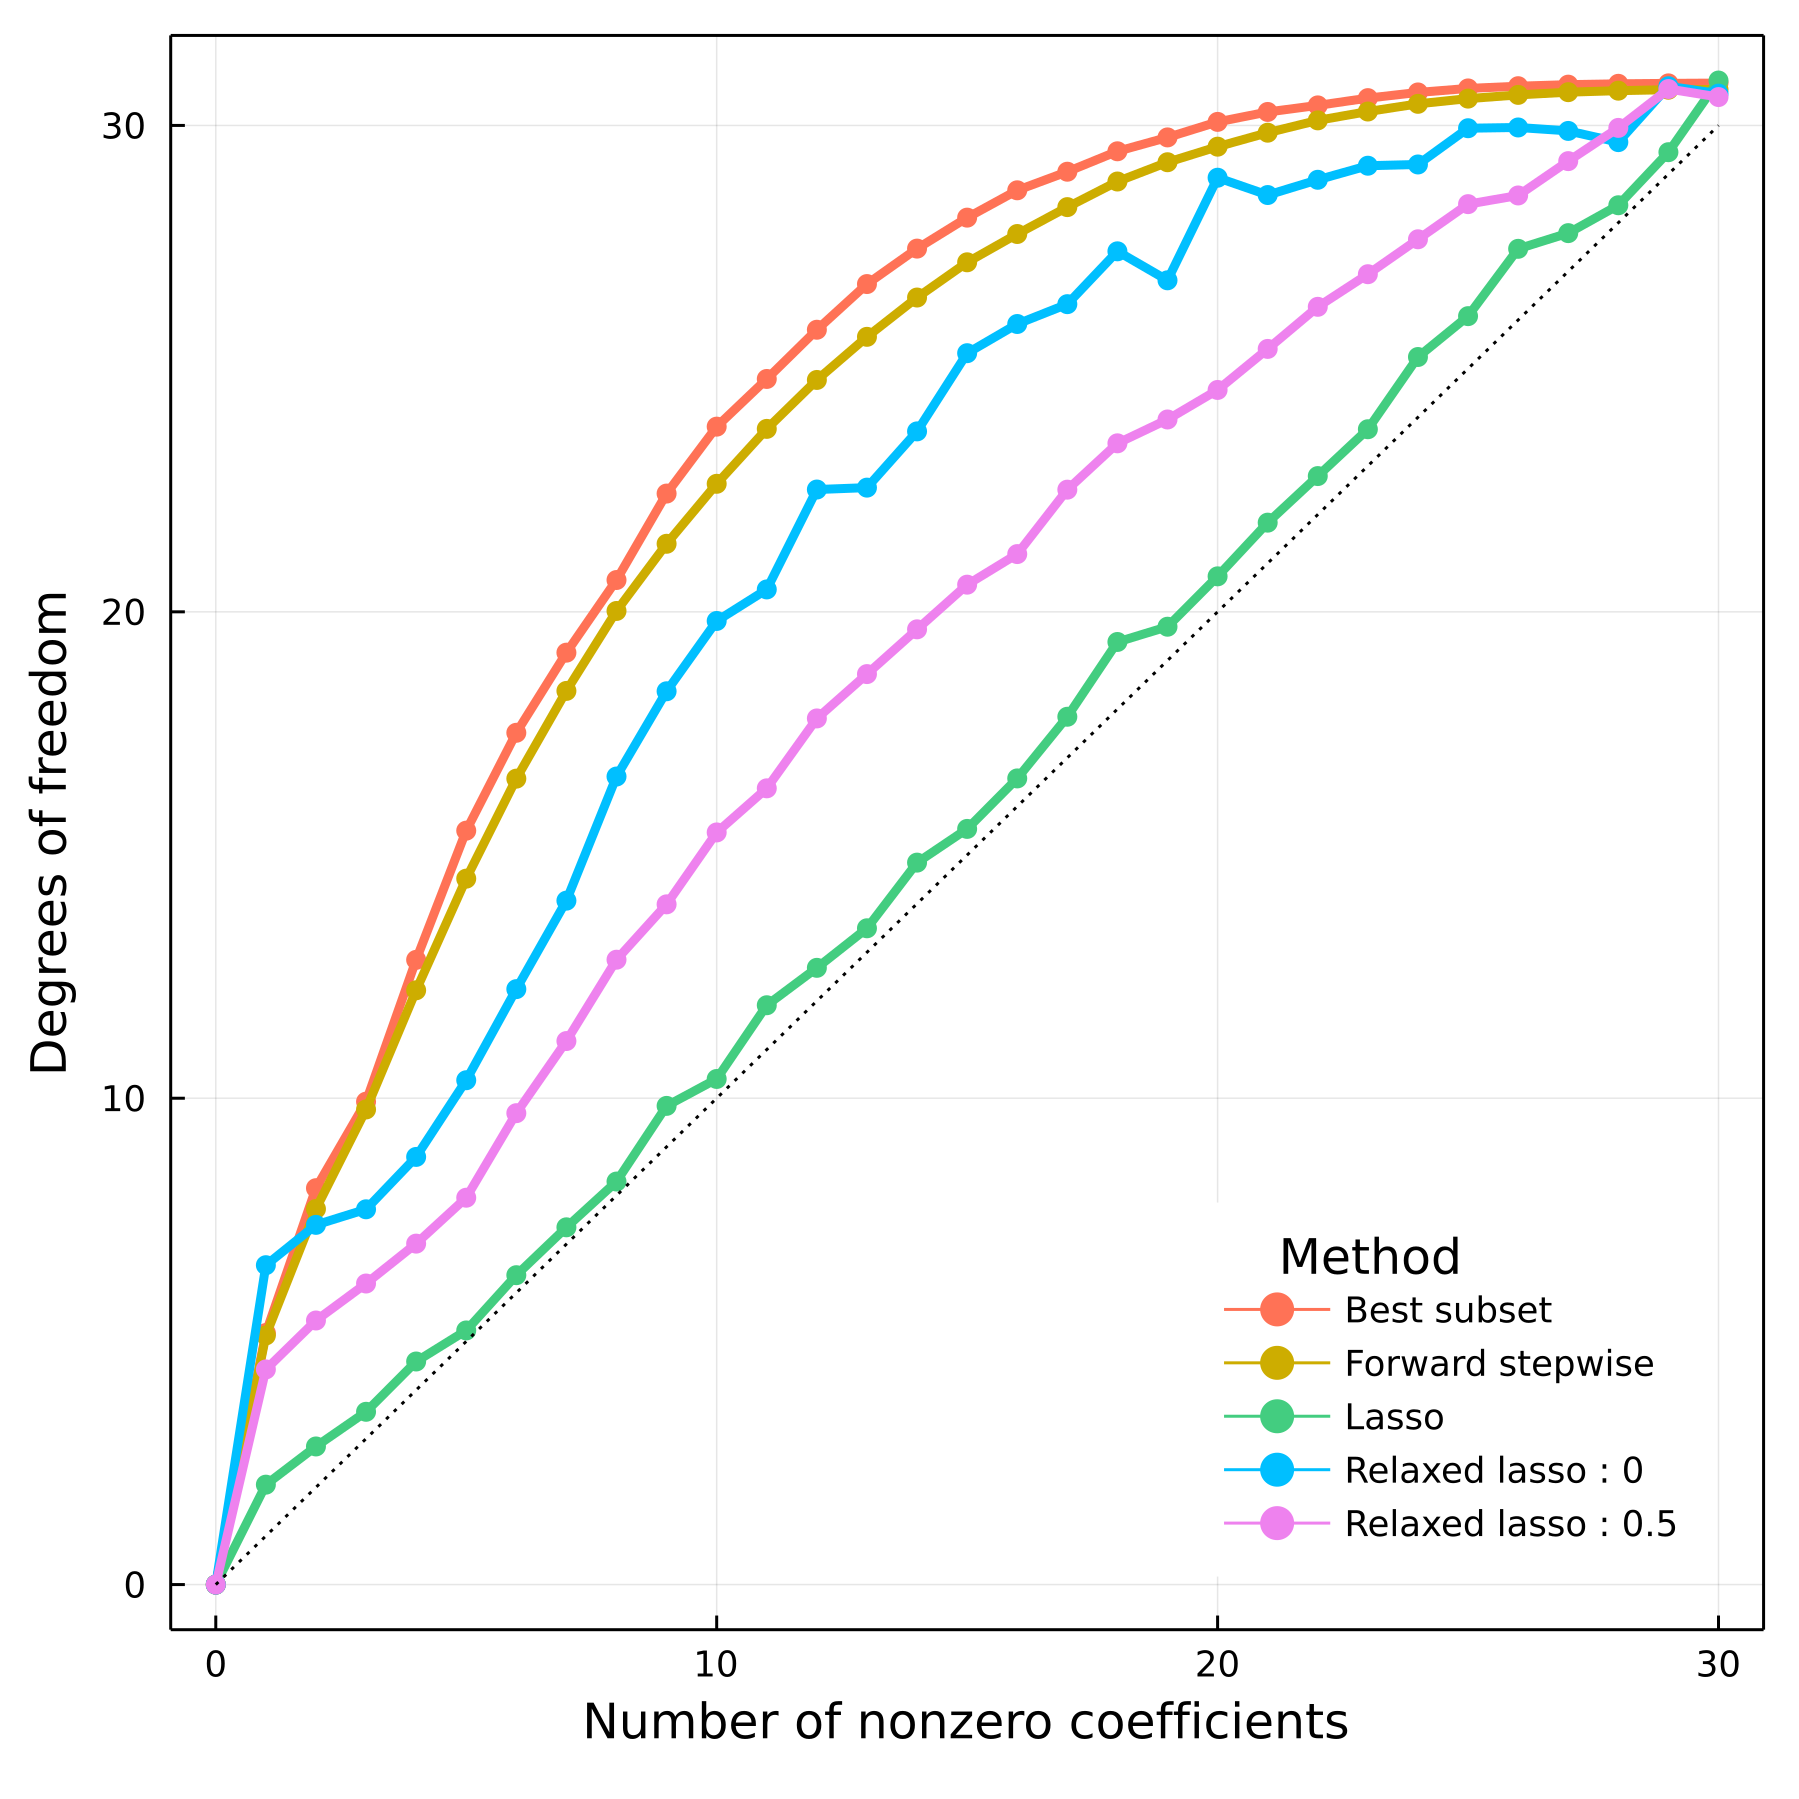
\includegraphics[width=0.475\linewidth]{./images/Figure 4.png}
    \caption{Degrees of freedom $\sum_{i=1}^n Cov(Y_i, \hat{Y}_i) / \sigma^2$ for the lasso, forward stepwise, best subset and the relaxed lasso with $\gamma = 0.5$ and $\gamma = 0$.}
  \end{figure}

\end{frame}


\begin{frame}{Results: Accuracy Metrics (Low)}

  \begin{figure}
    \centering
    \includegraphics[width=0.75\linewidth]{./images/fig5.png}
    \caption{RTE, PVE, number of nonzero coefficients and F-score as functions of SNR with $n = 100, p = 10, s = 5, \rho = 0.35$ and beta-type 2.}
  \end{figure}

\end{frame}


\begin{frame}{Results: Accuracy Metrics (Low)}

  \begin{figure}
    \centering
    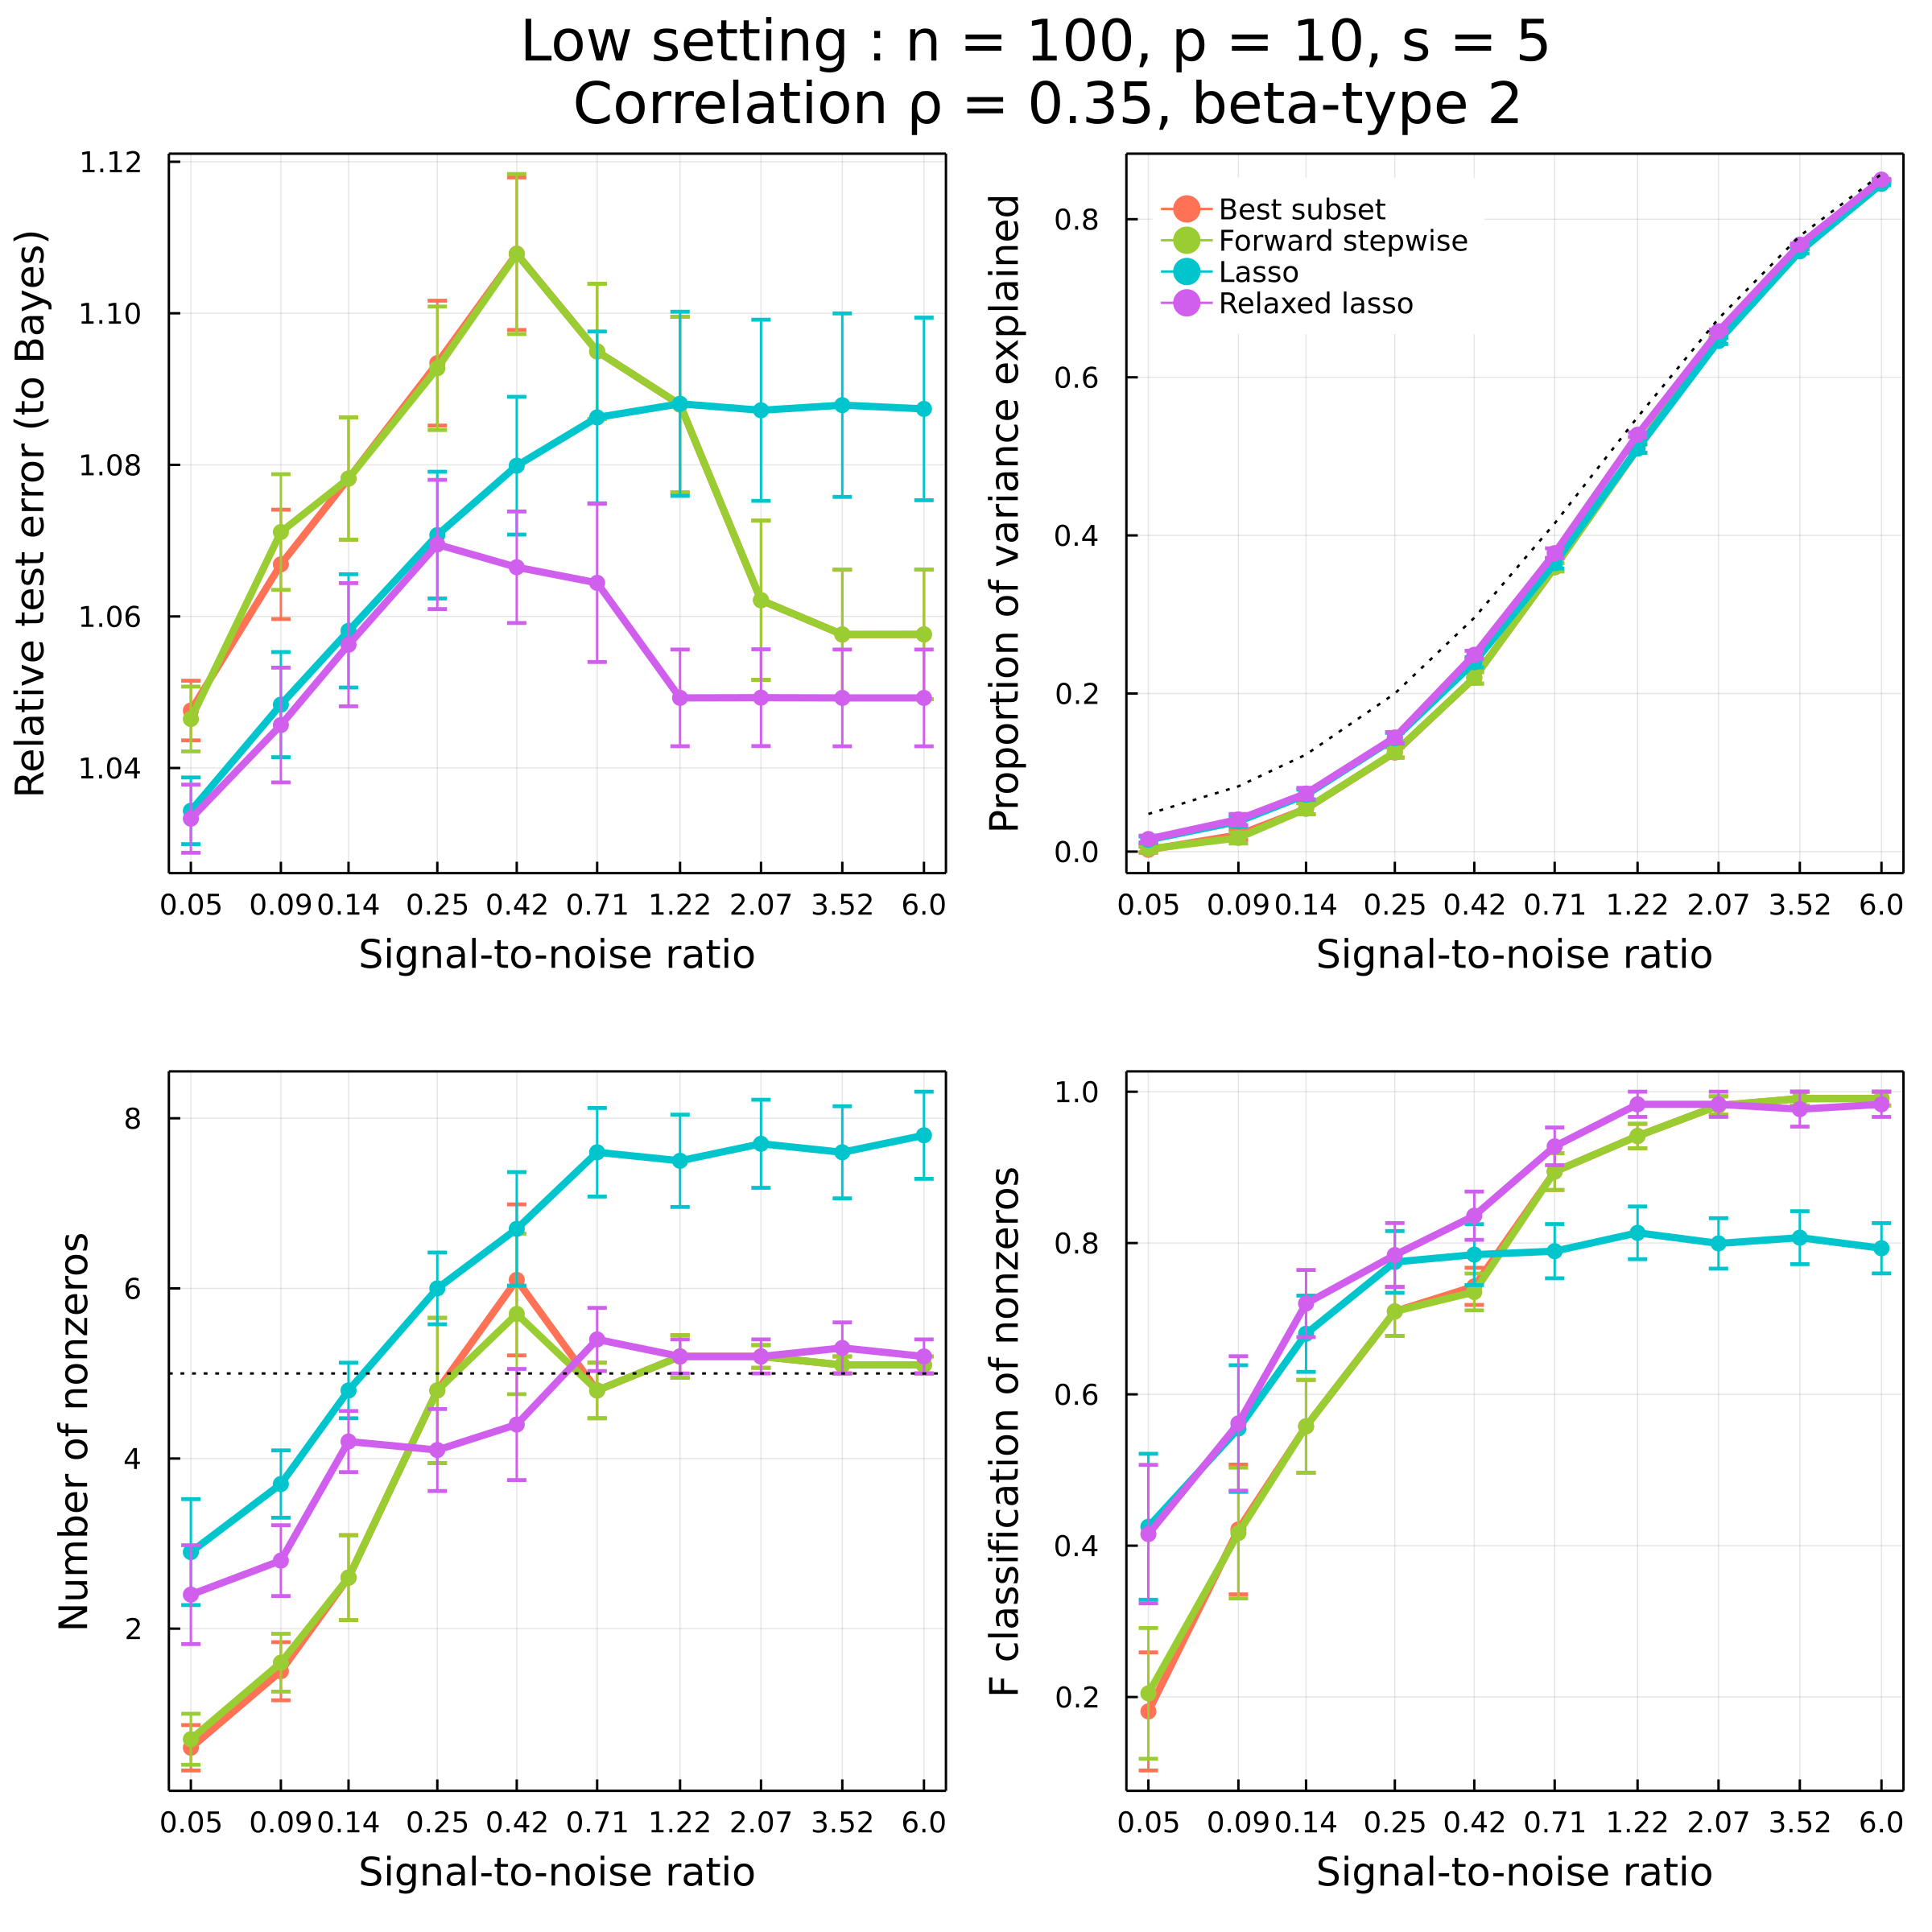
\includegraphics[width=0.75\linewidth]{./images/Figure 5.png}
  \end{figure}

\end{frame}


\begin{frame}{Results: Accuracy Metrics (Medium)}

  \begin{figure}
    \centering
    \includegraphics[width=0.75\linewidth]{./images/fig6.png}
    \caption{RTE, PVE, number of nonzero coefficients and F-score as functions of SNR with $n = 500, p = 100, s = 5, \rho = 0.35$ and beta-type 2.}
  \end{figure}

\end{frame}


\begin{frame}{Results: Accuracy Metrics (Medium)}

  \begin{figure}
    \centering
    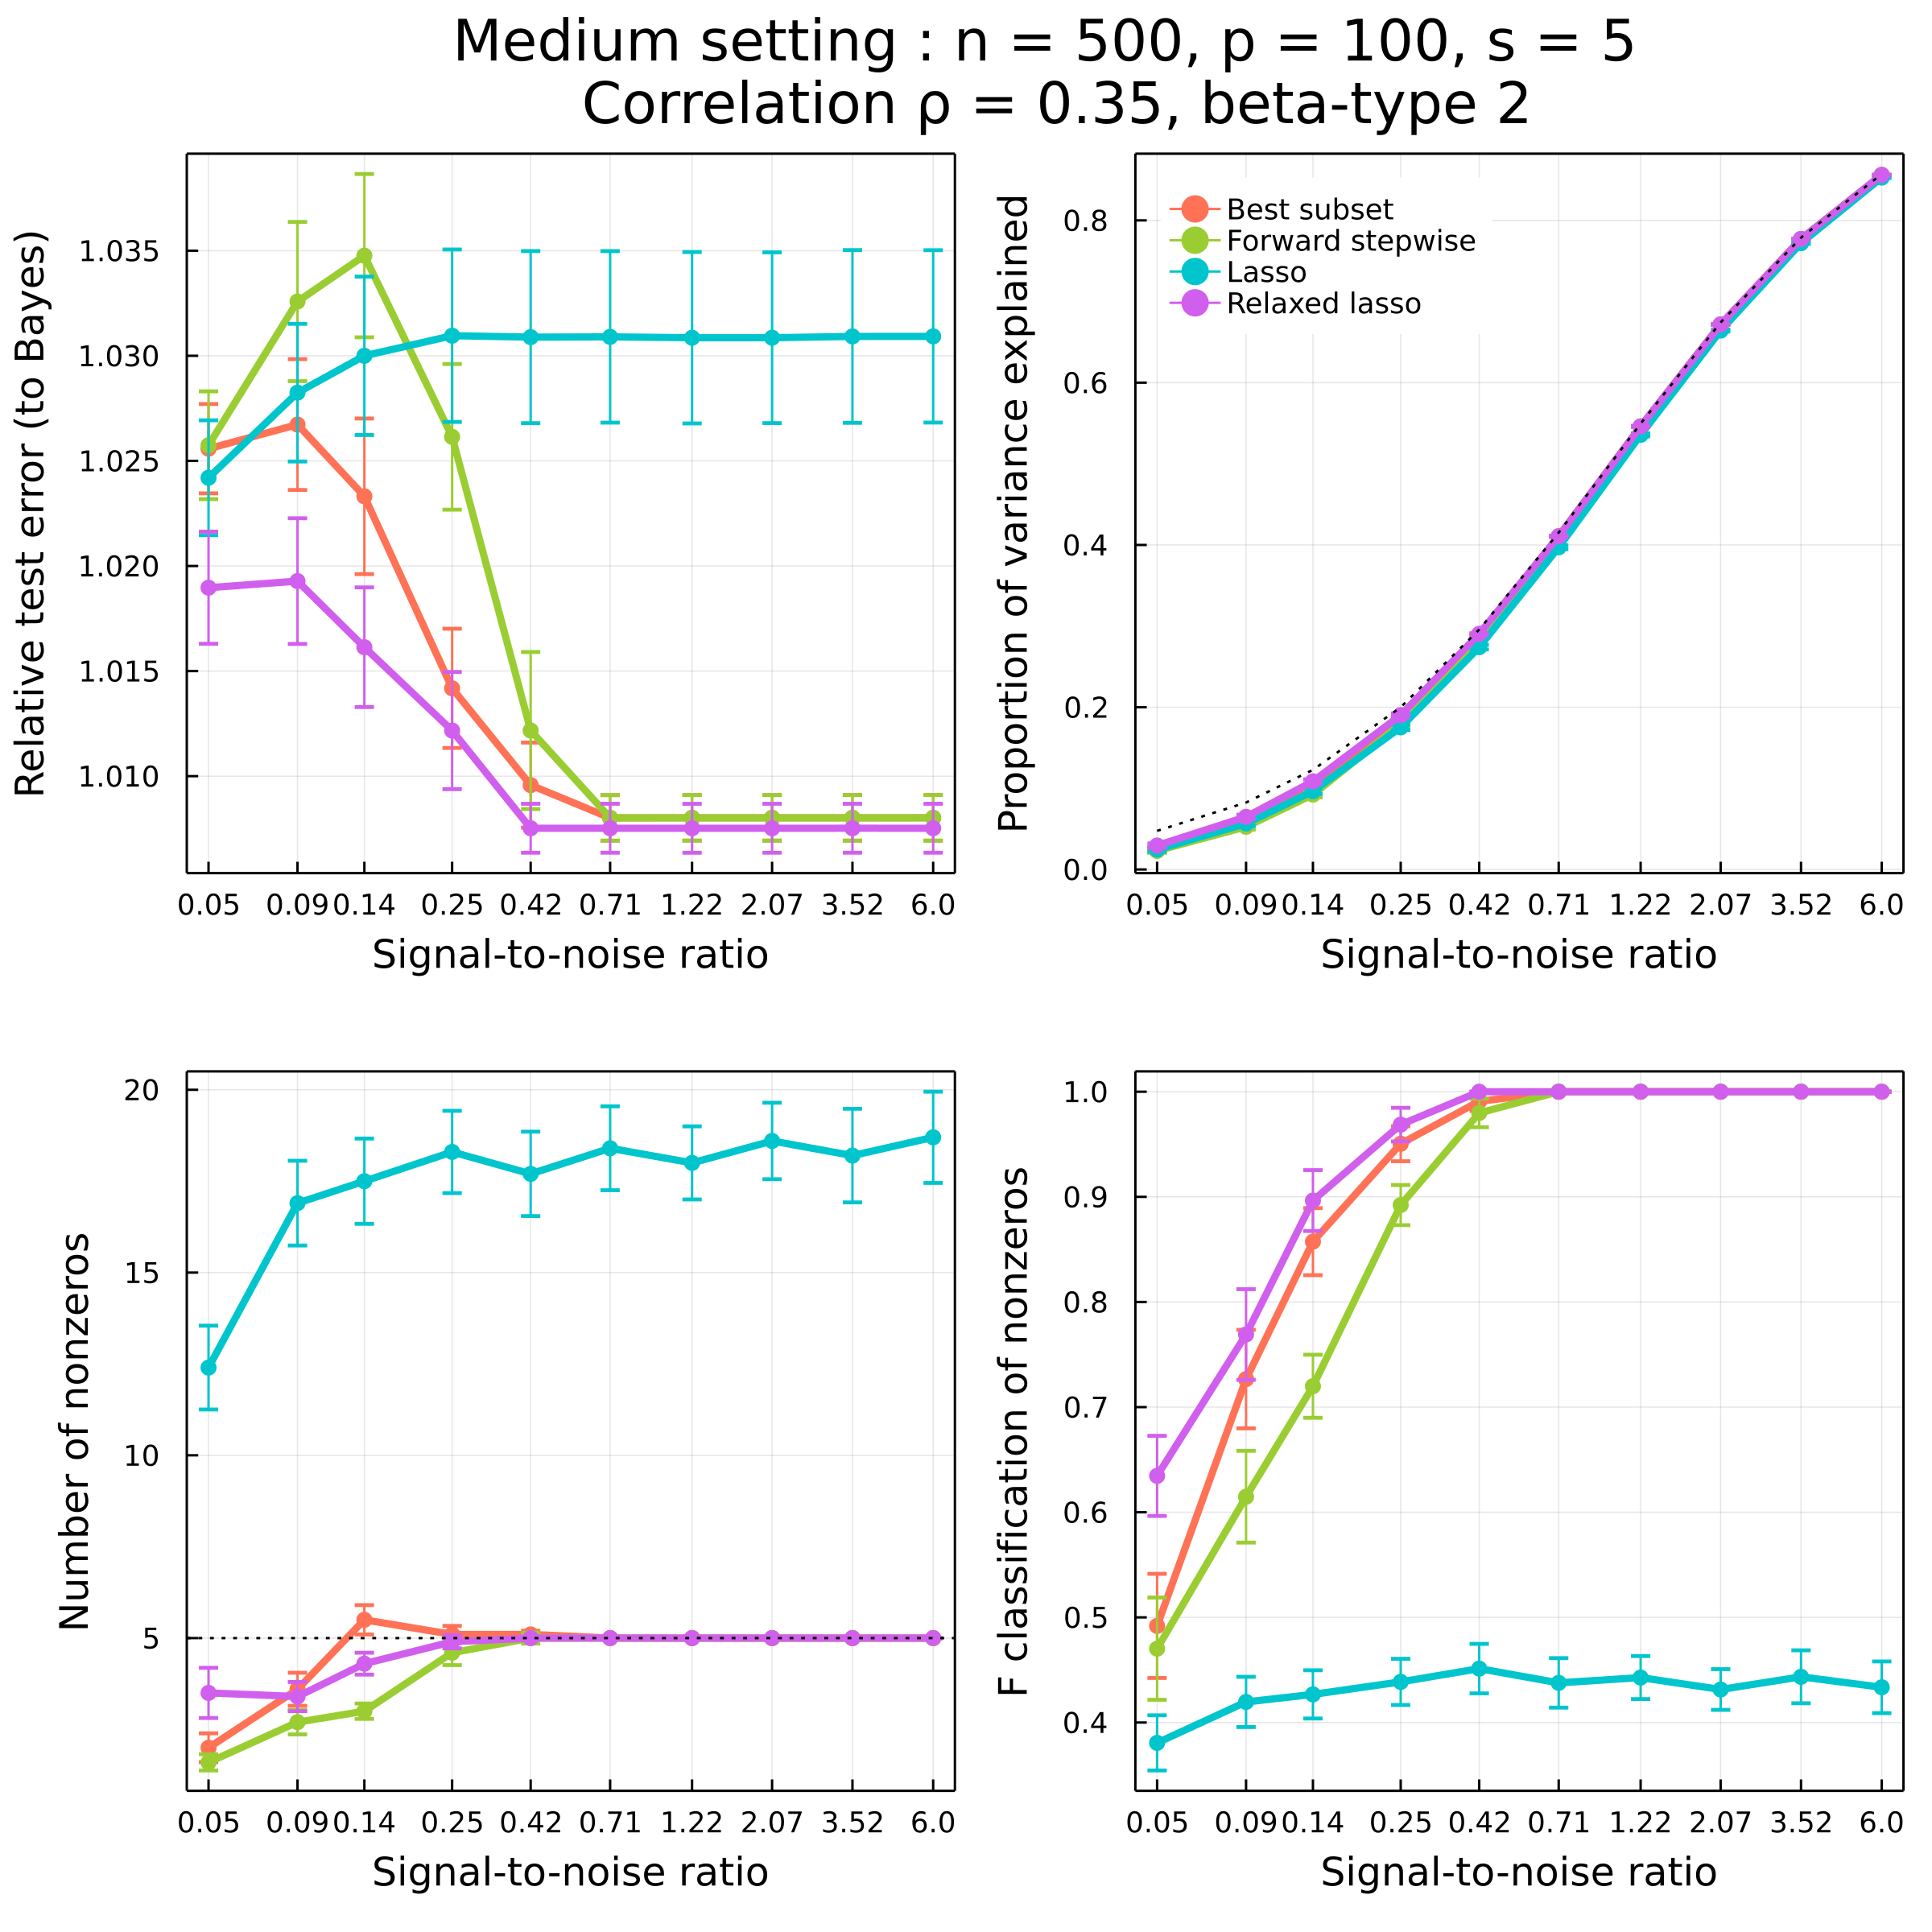
\includegraphics[width=0.75\linewidth]{./images/Figure 6.png}
  \end{figure}

\end{frame}


\begin{frame}{Results: Accuracy Metrics (High-5)}

  \begin{figure}
    \centering
    \includegraphics[width=0.75\linewidth]{./images/fig7.png}
    \caption{RTE, PVE, number of nonzero coefficients and F-score as functions of SNR with $n = 50, p = 1000, s = 5, \rho = 0.35$ and beta-type 2.}
  \end{figure}

\end{frame}


\begin{frame}{Results: Accuracy Metrics (High-5)}

  \begin{figure}
    \centering
    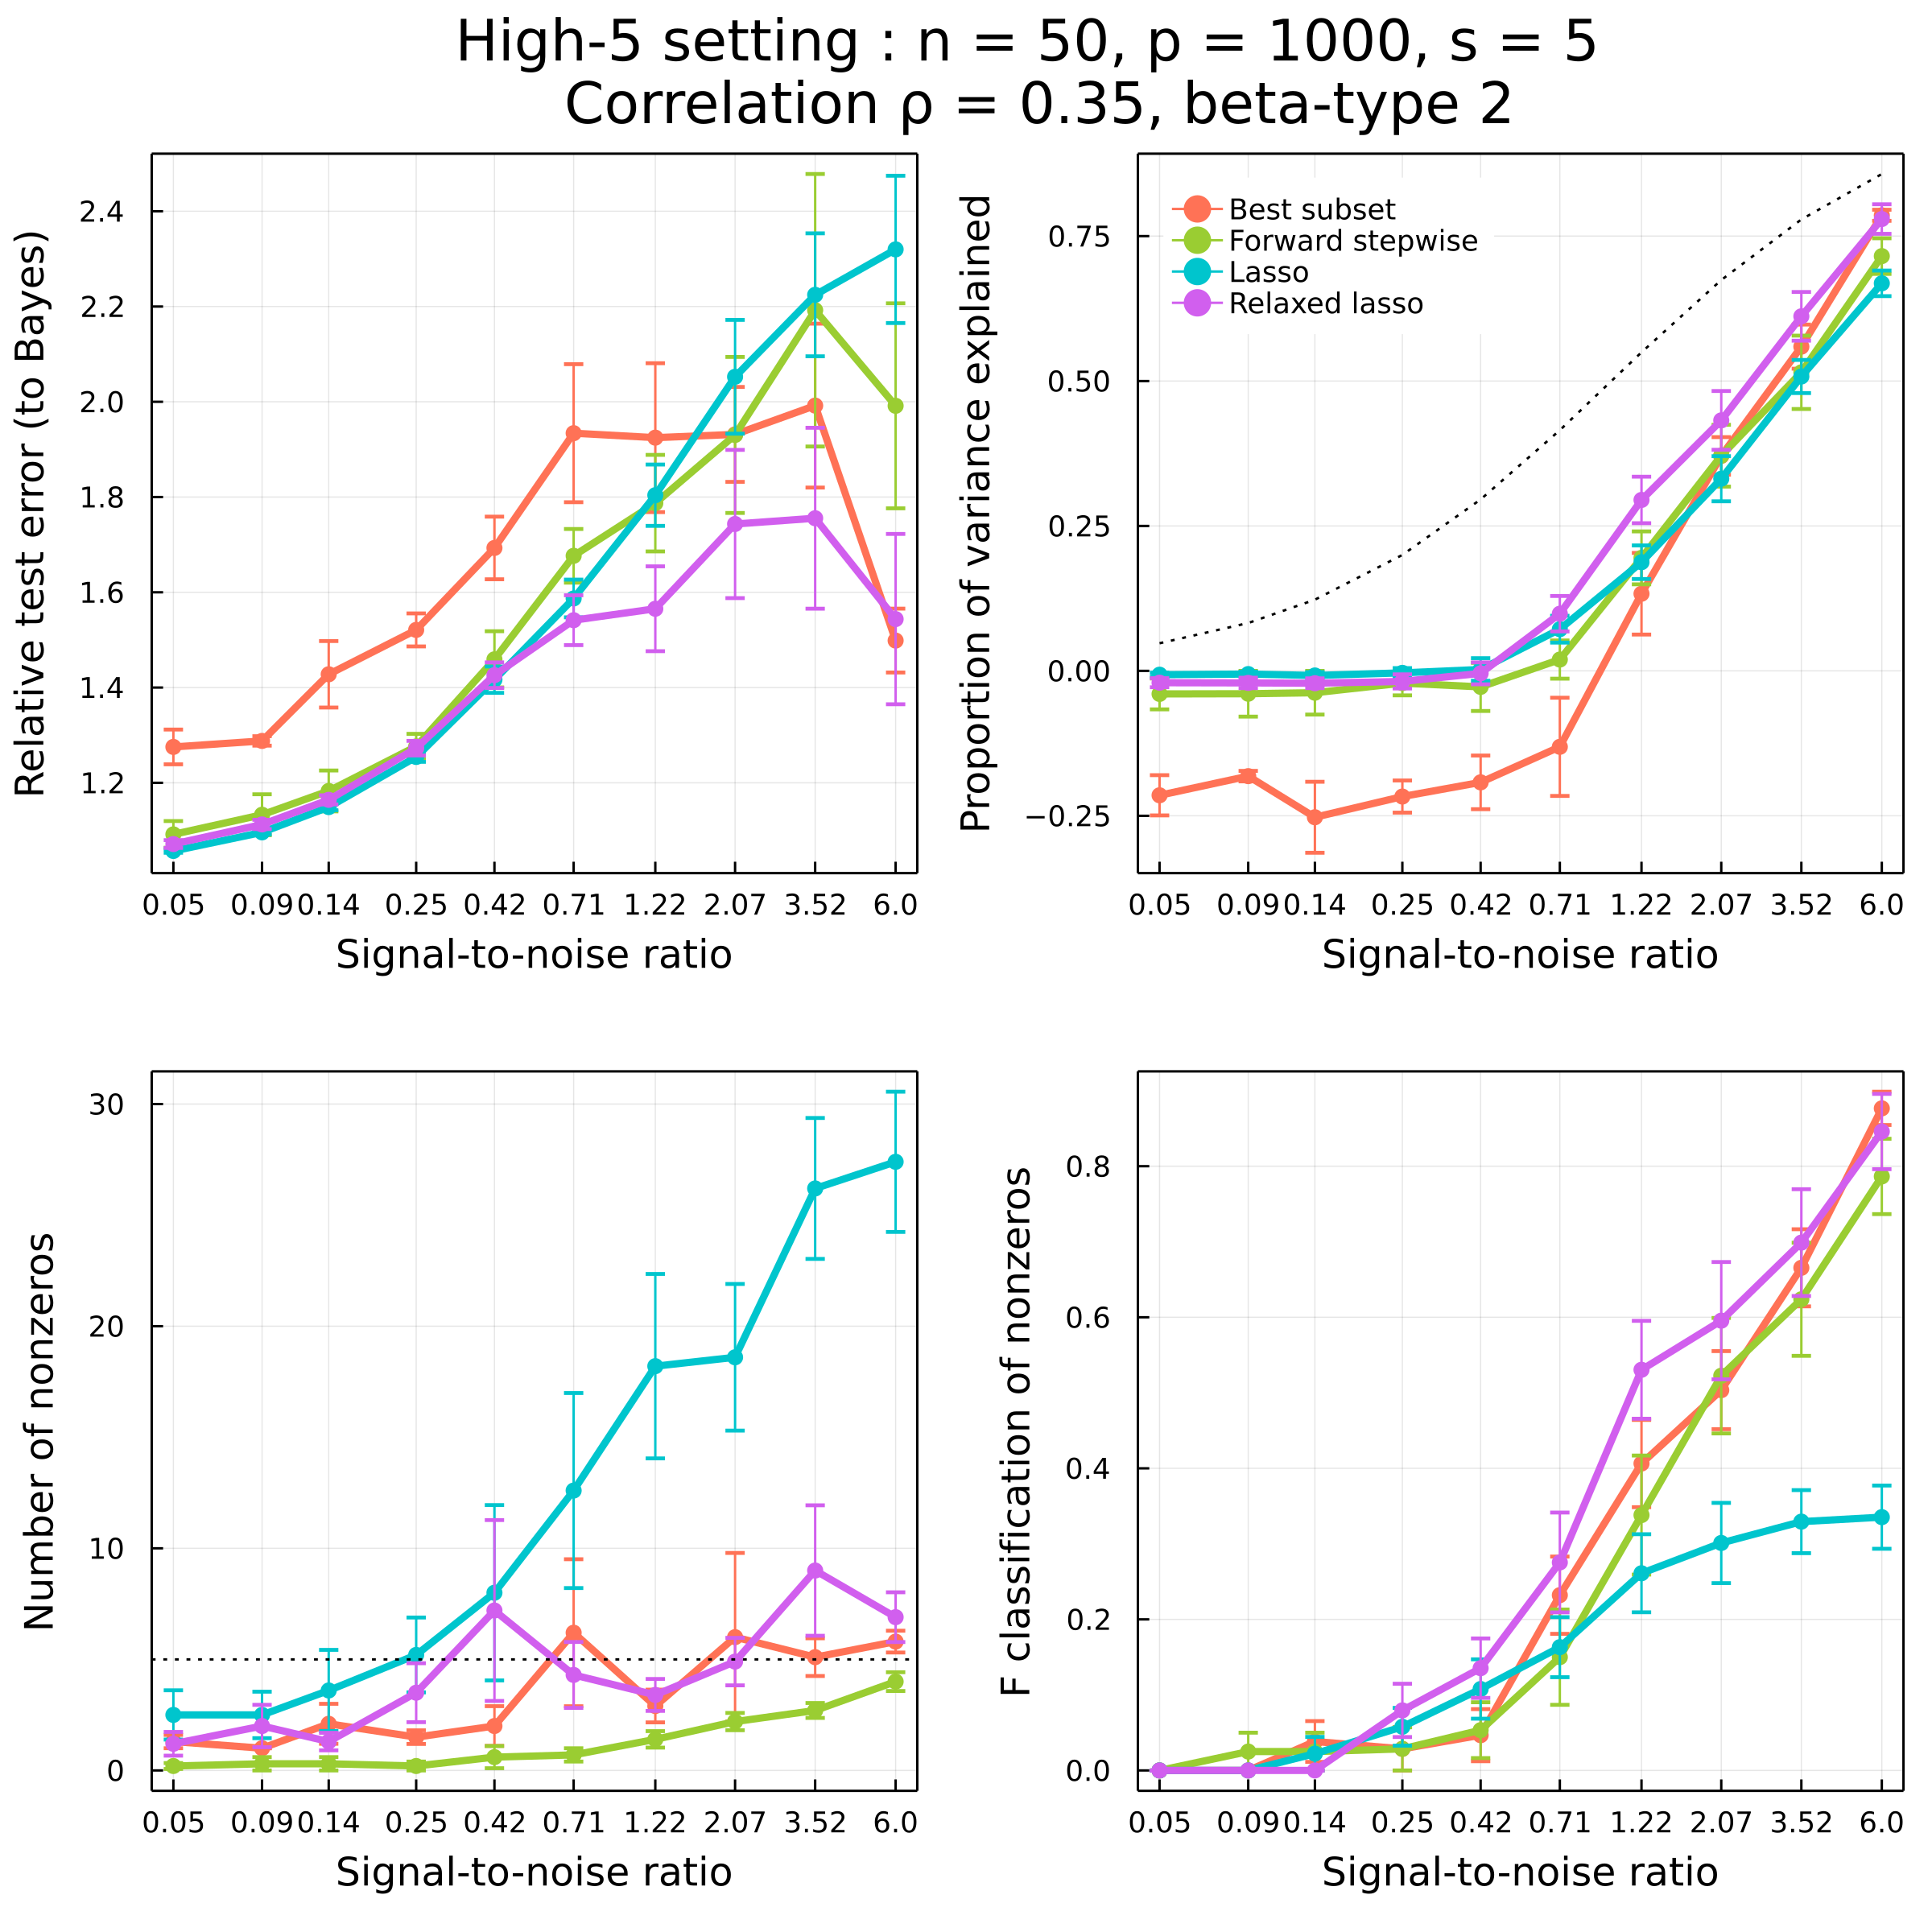
\includegraphics[width=0.75\linewidth]{./images/Figure 7.png}
  \end{figure}

\end{frame}


\begin{frame}{Results: Accuracy Metrics (High-5)}

  \begin{figure}
    \centering
    \includegraphics[width=0.75\linewidth]{./images/fig8.png}
    \caption{RTE, PVE, number of nonzero coefficients and F-score as functions of SNR with $n = 50, p = 1000, s = 5, \rho = 0.35$ and beta-type 1.}
  \end{figure}

\end{frame}


\begin{frame}{Results: Accuracy Metrics (High-5)}

  \begin{figure}
    \centering
    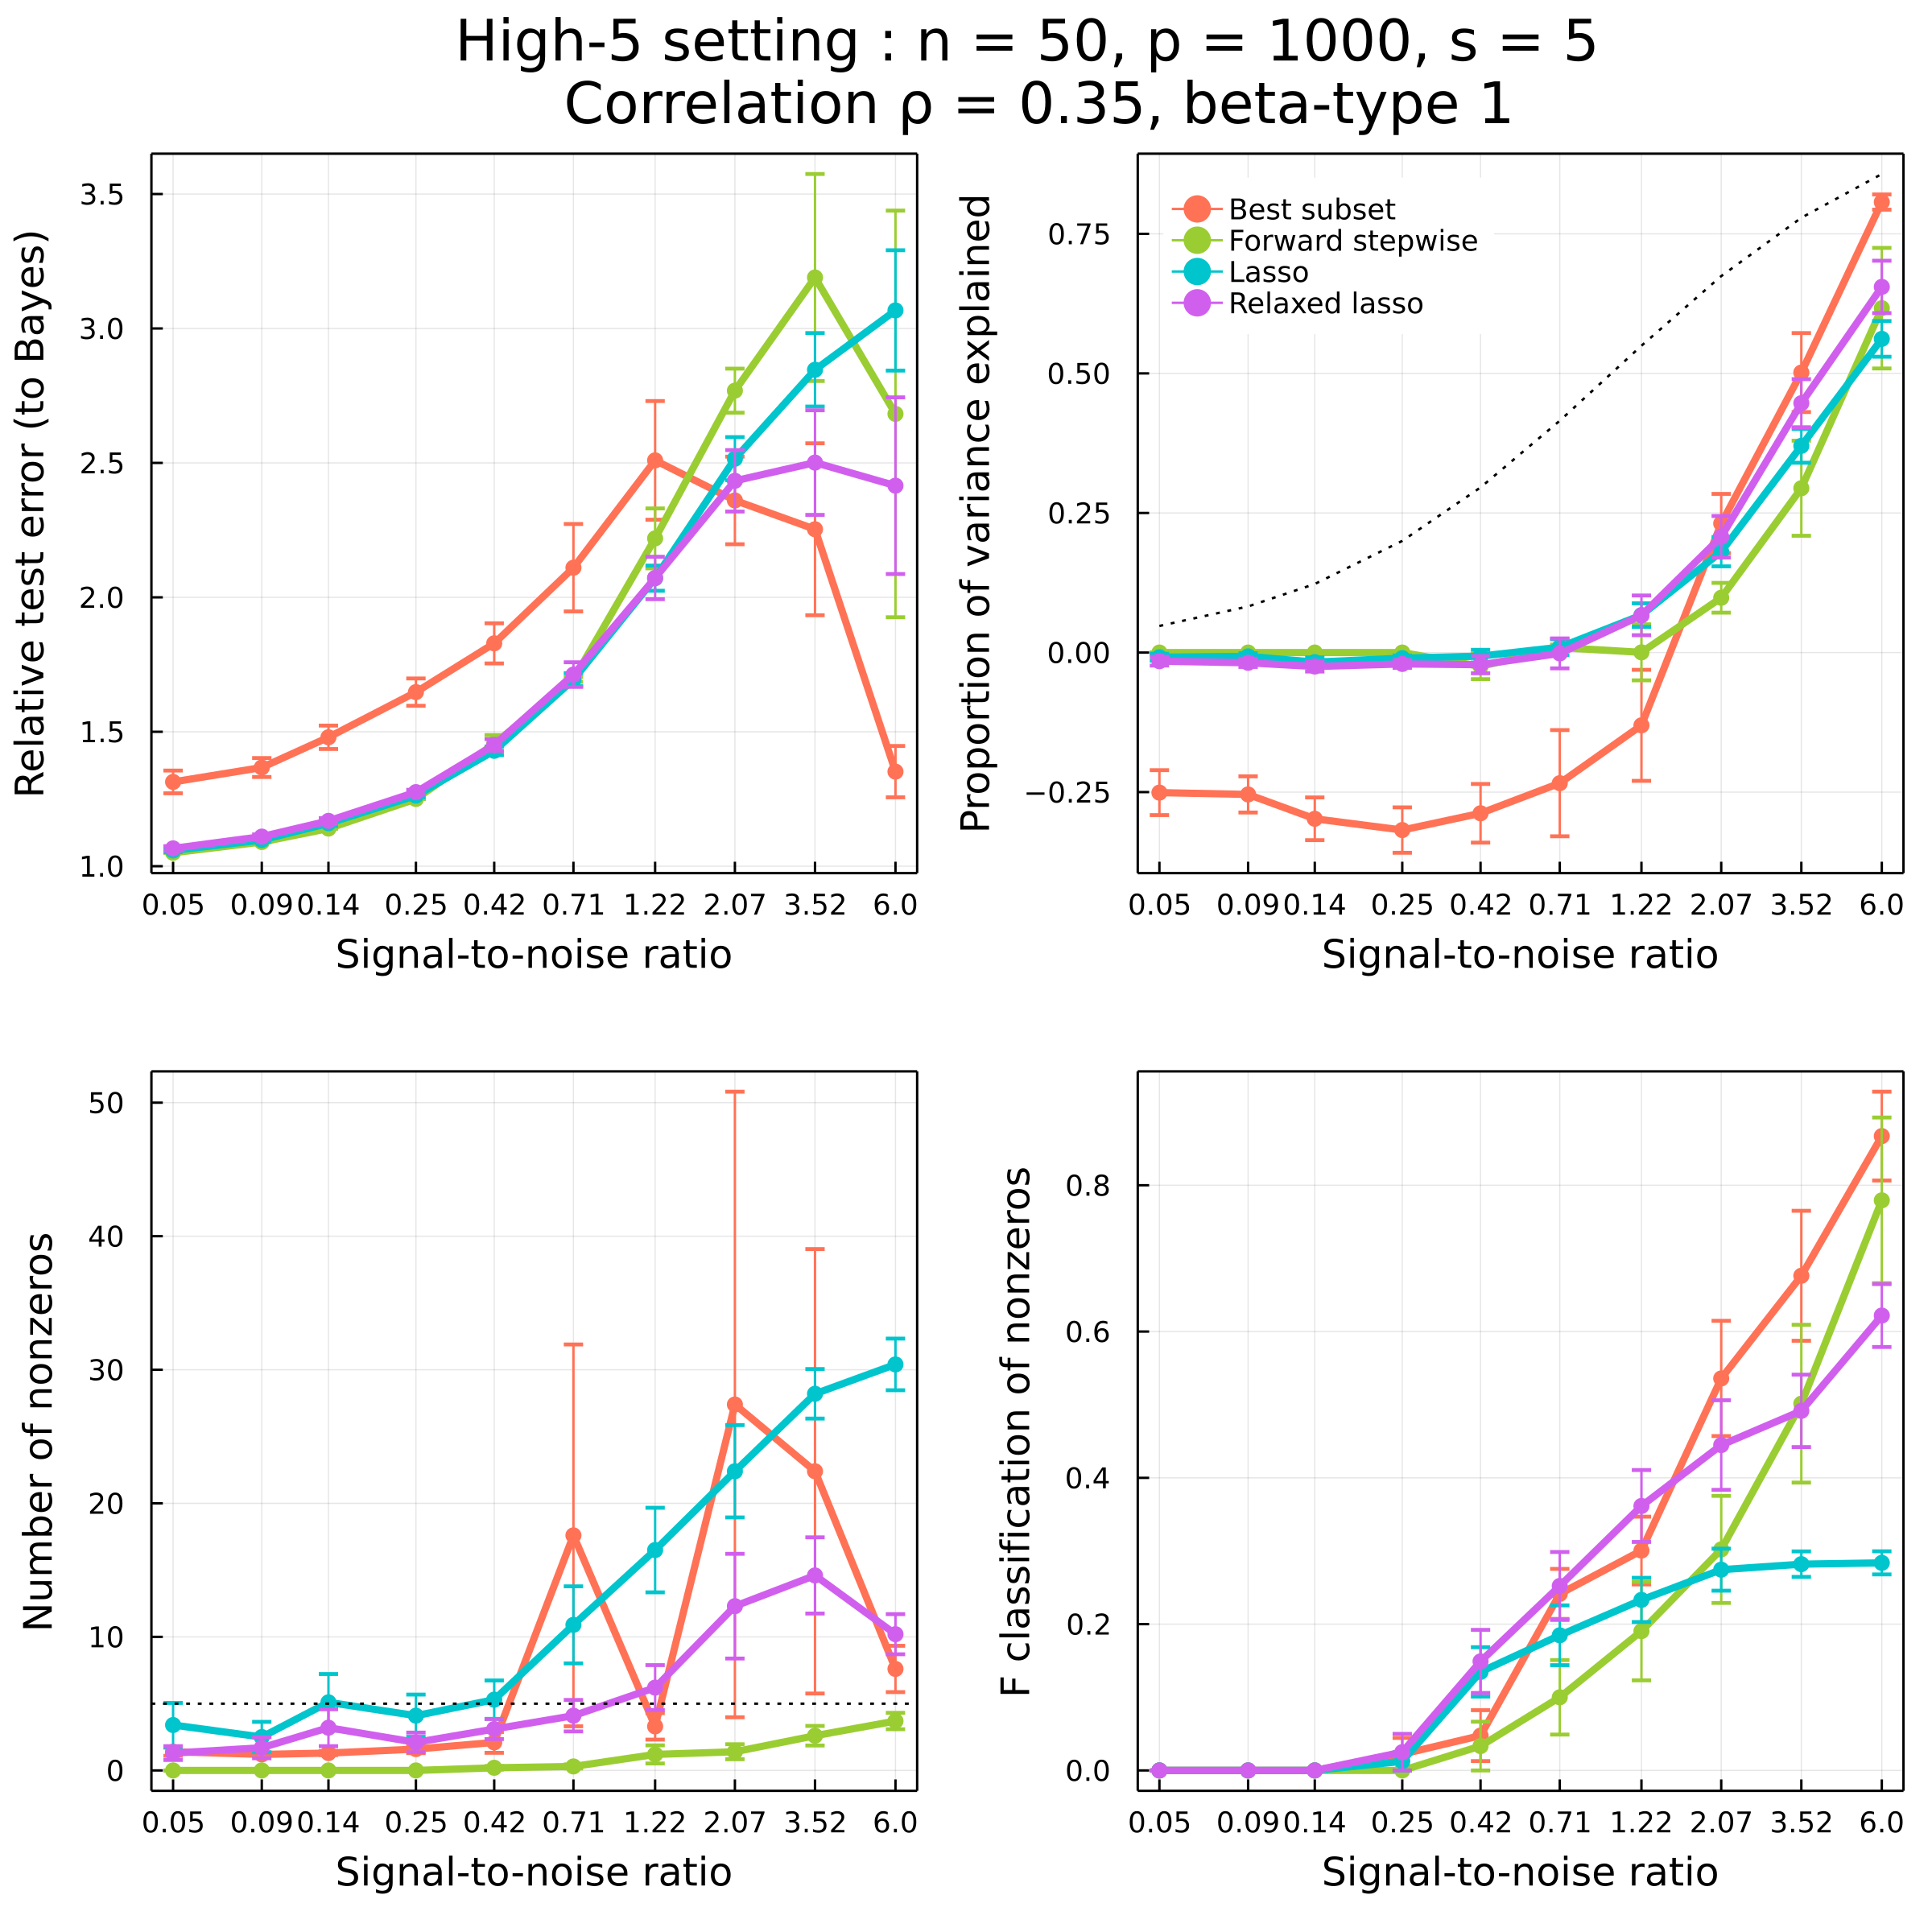
\includegraphics[width=0.75\linewidth]{./images/Figure 8.png}
  \end{figure}

\end{frame}


\begin{frame}{Summary of Results}

  \begin{itemize}
    \item The lasso and relaxed lasso are very fast and forward stepwise is also fast, though not quite as fast as the lasso.
    \item In high-5 and high-10 setting, best subset selection gives very poor accuracy because of time-limit.
    \item Forward stepwise selection and best subset selection perform quite similarly over all settings, but the former one is much faster.
    % This does not agree with the results for forward stepwise in Bertsimas et al (2016).
    \item In the low SNR range, the lasso outperforms the best subset selection while it has worse accuracy than best subset selection in the high SNR range.
    \item The relaxed lasso performs better than all other methods over all settings.
  \end{itemize}

\end{frame}


\begin{frame}{References}

  \begin{itemize}
    \item Hastie, T., Tibshirani, R. and Tibshirani, R. (2020). Best Subset, Forward Stepwise or Lasso? Analysis and Recommendations Based on Extensive Comparisons. \textit{Statistical Science}. \textbf{35} 579-592.
    \item Bertsimas, D., King, A. and Mazumder, R. (2016). Best subset selection via a modern optimization lens. \textit{The Annals of Statistics}. \textbf{44} 813-852.
    \item Tibshirani, R., Bien, J., Friedman, J., Hastie, T., Simon, N., Taylor, J and Tibshirani, R. (2012). Strong rules for discarding predictors in lasso-type problems. \textit{Journal of the Royal Statistics Society}. \textbf{74} 245-266.
    \item Friedman, J., Hastie, T., Hofling, H. and Tibshirani, R. (2007). Pathwise Coordinate Optimization. \textit{The Annals of Statistics}. \textbf{1} 302-332.
  \end{itemize}

\end{frame}
%--------------------------------------------------
\end{document}